\chapter{Graphical Neural Network}

\section{Primer}
Recall for node embeddings, we want to map node to a $d$ dimensional embeddings such that similarity(decoder) of those two embeddings are close for nodes close to each other. Now we use deep graph encoders. This can solve 
    \begin{itemize}
        \item node classification 
        \item link prediction 
        \item community detection 
        \item network similarity 
    \end{itemize}
    

\section{Deep Learning for Graphs Requirement}
\paragraph{Setup} \mbox{}\\
Assume we have a graph $G$: 
    \begin{itemize}
        \item $V$ is the vertex set 
        \item $A$ is the adjacency matrix 
        \item $X\in \mathbb{R}^{m \times |V|}$ is a amtrix of node feature 
        \item $v$ is a node in $V$. $N(v)$ is the neighbors. 
    \end{itemize}
Notice for a given graph, we have many ordering plans for the nodes. So our algorithm has to be invariance / equivariance. 

\paragraph{Permutation Invariance and Equivariance} \mbox{}\\
Let $f$ be a function that maps a graph $G=(A,X)$ to a vector $\mathbb{R}^d$. Then we say $f$ is permutation invariant function if we can shuffle the order of the columns of $A$ and $X$ (i.e.: different order plan for nodes). \\

Let $f$ be a function that maps a graph $G=(A,X)$ to $\mathbb{R}^{m \times d}$ where $m$ is the number of nodes. The output each row is the embedding of a node. We say $f$ is equivariance if we can shuffle the order of the input, and the embedding output for the same node is the same. 



\section{Graph Convolutional Networks - Basic Approach} 
Idea: We let a node's neighborhood defines a computation graph. So below is an example of a 2 layer GNN setup for a specific node. Each node will have a computation graph. 
    \begin{figure}[h]
    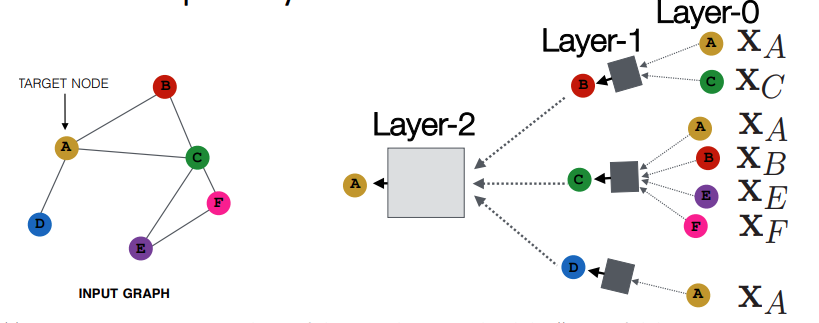
\includegraphics[width=12cm, height=6cm]{images/003_two_layer_GNN.png}
    \end{figure}

So we have a two step process at each layer: 1) average messages from neighbors and 2) apply neural network. 
    \begin{align*}
        & h_v^0 = x_v \tag{Initial 0-th layer embeddings are equal to node features} \\
        & h_v^{k+1} = \sigma(W_k \sum_{u\in N(v)} \frac{h_u^{(k)}}{|N(V)|} + B_k h_v^{(k)}) & \forall k\in \{ 0, ..., K-1\}\\
        & z_v = h_v^{K}
    \end{align*}
    \begin{itemize}
        \item $\sum_{u\in N(v)} \frac{h_u^{(k)}}{|N(V)|}$ is averaging the embeddings of neighbors. (This is order invariant)
        \item $B_k h_v^{(k)}$ is just the embedding of the same node in $k$ layer. 
        \item $\sigma$ is an activation function 
        \item $W_k$ is shared across all nodes. $W$ is only different at different layer. 
        \item We can also think of the process as $\sum_{u\in N(v)} W_k\frac{h_u^{(k)}}{|N(V)|}$. So each neighbor's message for layer $k+1$ is computed as $ W_k\frac{h_u^{(k)}}{|N(V)|}$, and the aggregation process is a sum. 
    \end{itemize}


\section{Matrix Formulation of the simple GNN with average aggregation } 
Many aggregations can be performed efficiently by sparse matrix operations. 
    \begin{align*}
        & \textrm{Let } H^{(k)}=[h_1, ..., h_{|v|}^{(k)}]^T\\
        & \Longrightarrow \sum_{u\in N_v} h_u^{(k)} = A_v H^{(k)} \tag{$A_v$ is the row for node $v$ in adjacency matrix} \\
        & \textrm{Let $D$ be a diagonal matrix and  } D_{v,v} = Deg(v) = |N(v)|\\
        & \Longrightarrow  H^{(k+1)} = \sigma(D^{-1}AH^{(k)}W_k^T + H^{(k)}B_k^T)\\
    \end{align*}
    
\section{Training Simple GNN} 
The mode parameters are $W_i$ and $B_i$. I will have one $W$ and one $B$ per layer. So we just need to decide a loss function. \\
For supervised learning, the node embedding $z_v$ is a function of input graph. We can try to minimize the loss $L(y, f(z_v)$ \\
In an unsupervised setting, we can use the graph structure as the supervision. Hence $L = \sum_{z_w, z_v} CE(y_{u,v}, DEC(z_u, z_v))$. The CE is cross entropy. DEC is decoder such as inner product. We can set $y_{u,v}=1$ when node $u$ and $v$ are similar, and node similarity can be anything from previous lecture such as random walks.  


\section{GNN Component Summary}
In a general GNN framework, we have 4 components: 
    \begin{itemize}
        \item Messaging + Aggregation 
        \item Layer Connectivity
        \item Graph Augmentation (input graph $\neq$ computational graph): graph feature augmentation, graph structure augmentation 
        \item Learning objective: supervised vs. unsupversed, node/edge/graph level objectives
    \end{itemize}
    

\section{Single Layer of GNN}
Single layer of GNN has two component: 
\paragraph{Message Computation} \mbox{}\\
Each node will create a message, which will be sent to other nodes later: 
    \begin{align*}
        m_u^{(l)} = MSG^{{l}}(h_u^{(l-1)}
    \end{align*}
Some example could be a linear layer  $m_u^{(l)} = W^{(l)}h_u^{(l-1)}$. \\
In addition, we want to compute a different message for the node $v$ itself, that will be used for self node's message at next layer: 
    \begin{align*}
        m_v^{(l)} = MSG(h_v^{(l-1)}) = B^{(l)}h_v^{(l-1)} \tag{example of linear embedding}
    \end{align*}

\paragraph{Aggregation} \mbox{}\\
Node $v$ will aggregate the message from node $v$'s neighbors as well as the message from itself from previous layer. 
    \begin{align*}
        h_v^{(l)} = AGG^{(l)}(\{m_u^{(l)}, u\in N(v) \}, m_v^{(l)})
    \end{align*}
The aggregation could be using sum, mean, max and etc. The way to incorporate self message could be through concatenation, or aggregation. 


\subsection{GraphSAGE Layer}
    \begin{align*}
        h_v^{(l)} = \sigma \left( W^{(l)} \cdot CONCAT\left(h_v^{(l-1)}, AGG(\{ h_u^{(l-1)}, \forall u\in N(v)  \})\right)  \right)
    \end{align*}
    \begin{itemize}
        \item Message is computed within the $AGG(\cdot)$
        \item First we aggregate from node neighbors, $AGG(\{ h_u^{(l-1)}, \forall u\in N(v)  \})$
        \item then we further aggregate over the node itself through concatenation 
    \end{itemize}
Different kind of aggregator: 
    \begin{itemize}
        \item Mean: Take a weighted average of neighbors $AGG = \sum_{u\in N(v)} \frac{h_u^{(l-1)}}{|N(v)|}$
        \item Pool: Transform neighbor vectors (e.g.: Multilayer Perceptron) and apply symmetric vector function Mean or Max: $AGG = Mean\left( \{ MLP(h_u^{(l-1)}), \forall u \in N(v)    \} \right)$
        \item LSTM: Apply LSTM to \textbf{reshuffled} of neighbors (so model doesn't learn the sequence) $AGG = LSTM([h_u^{(l-1)}, \forall u \in N(v)]$
    \end{itemize}

L2 Normalization: 
    \begin{itemize}
        \item We can apply l2 normalization to $h_v^{(l)}$ at every layer
    \end{itemize}
    
    
\subsection{Graph Attention Networks Layer}
We can have an weight factor for each edge $a_{vu}$
    \begin{align*}
        h_v^{(l)} = \sigma(\sum_{u \in N(v)} a_{vu} W^{(l)}h_u^{(l-1)})
    \end{align*}
    \begin{itemize}
        \item In GCN / GraphSage, $a_{vu} = \frac{1}{|N(v)|}$ is the weighting factor of node $u'$ message to node $v$. All neighbors are equivalent important. 
        \item Ideally we want to let different neighbor have different attention
    \end{itemize}
Overall, we want to let the attention $a_{vu}$ be computed as a byproduct of an attention mechanism function $\alpha$
    \begin{align*}
        & \textrm{First we compute attention coefficient based on messages} \\
        & e_{vu} = \alpha(W^{(l)}h_u^{(l-1)}, W^{(l)}h_v^{(l-1)})\\
        & \textrm{Normalize $e_{vu}$ into the final attention weight with softmax}\\
        & a_{vu} = \frac{\exp(e_{vu})}{\sum_{k\in N(v)} \exp(e_{vk})}
    \end{align*}
The approach for attention mechanism function $\alpha$ can be a simple single layer neural network, e.g.: (The parameters of $\alpha$ are trained jointly with other parameters in end-to-end function. ) 
    \begin{align*}
        \alpha(W^{(l)}h_u^{(l-1)}, W^{(l)}h_v^{(l-1)}) = Linear(Concat(W^{(l)}h_u^{(l-1)}, W^{(l)}h_v^{(l-1)}))
    \end{align*}

Multi-head attention: Stablizes the learning process of attention mechanism. We create multiple attention scores, each generate a new $h_u^{(l1)}$, and then we can have an aggregation function to aggregate all different version of the message, such as sum, concatenation, or average. 





\section{Layer Connectivity}
Traditionally, we can construct Graph Neural Network just by stacking GNN layer sequentially. The input is the initial raw node feature $x_v$ and the output is the node embeddings $h_v^{L}$ after $L$ GNN layers. 

\paragraph{Over-smoothing}\mbox{}\\
\textbf{Receptive field} is a set of nodes that determine the embeddings of a node of interest. So for a two layer GNN, the receptive field is a node's 2 hop neighbors. As we add layer to GNN, there will be a lot of overlap in terms of receptive field, and thus eventually nodes embedding will converge to the same value. \\\par

Solution 1: We can make shallow GNN more expressive by making aggregation / transformation become a deep neural network. \\ \par

Solution 2: Add layers that do not pass messages. A GNN layer does not necessarily only contain GNN layer, we can add MLP layers (applied to each node) that does pre-process and post-process. \\ \par

Solution 3: Add skip connection in GNNs. So normally a standard GCN layer is $h_v^{(l)} = \sigma(\sum_{u \in N(v)} W^{(l)} \frac{h_u^{(l-1)}}{|N(v)})$, but now we have skipped connection: $h_v^{(l)} = \sigma(\sum_{u \in N(v)} W^{(l)} \frac{h_u^{(l-1)}}{|N(v)} + h_v^{(l-1)})$. Alternatively, we can also let the final layer directly aggregates from all the node embeddings in the previous layers. 


\section{Graph Augmentation} 
Our raw input graph doesn't have to be same as our computational graph. 
\subsection{Feature Augmentation}
If the input graph does not have node feature
    \begin{itemize}
        \item Assign a constant to each node: medium expressive power, inductive, and low computational cost.
        \item Assign unique ID to each node with one-hot encoding: highly expressive, not inductive, high computational cost due to $O(|V|)$ dimensitonal feature. 
    \end{itemize}
We can also strategically add certain structural features to node features, such as cycle length, PageRank, Centrality, Node degree, clustering coefficient. 

\subsection{Graph Structure Augmentation}
\subsubsection{Adding virtual nodes / edges}
To combat super sparse matrix, we can add virtual edges,
    \begin{itemize}
        \item Connect 2-hop neighbors via virtual edges (so instead of use GNN computation, we use $A + A^2$
        \item Just use the 2-hop virtual edges (This is especially useful for bipartie graphs. )
    \end{itemize}
We can also add virtual nodes that connect to all the nodes in the graph. Those nodes will improves message passing in sparse graphs 


\subsubsection{Sample neighbors when do message passing} 
If the graph is too dense, we can randomly sample a node's neighborhood for message passing. We can even use random walk to sample neighbors. 




\section{Learning Objective}
\subsection{Node-Level Prediction} 
After $GNN$ computation, we have $d$-dimensional node embeddings : $h_v^{(L)} \in \mathbbm{R}^d$. For classification, We can just wrap the head node with another matrix $W^H$ to map the embeddings to linear output and take softmax to compute loss. 


\subsection{Edge-Level Prediction}
We can make edge prediction by taking two head node. $\hat{y}_{u,v}= Head(h_u^{(L)}, h_v^{(L)})$. For design of the head function that aggregates, we can do 
    \begin{itemize}
        \item concatenation and then linear layer (not recommended)
        \item dot product for one-way prediction
        \item Multi-headed trainable matrix $W^{(1)}, ..., W^{(k)}$, $\hat{y}_{uv}^{(i)} = (h_u^{(l)})^TW^{(i)}h_v^{(l)}$ and then concatenate all the $\hat{y}^{(i)}$
    \end{itemize}


\subsection{Graph / Subgraph Level Prediction}
For graph level prediction of a smaller graph, we can think of it as aggregation over all embeddings, such as averaging, summing, maxing. For large graph, we can do hierarchically pooling. For example, we can use $RELU(Sum(\cdot))$. So we can divide nodes into different batches in hierarchically structure, run  $RELU(Sum(\cdot))$ on each batch, and then run $RELU(Sum(\cdot))$ on the result, and so on. DiffPool has two GNN, one to generate aggregate node, and one to create series of hierarchical cluster assignment. We can also do this many times and have two GNN for each layer of the aggregation. 


\subsection{Loss function} 
In supervised learning, we can use ground truth. In unsupervised learning, the signals come from graph themselves such as clustering coefficient. \\
For classification loss, we can use Cross Entropy loss in a K-way prediction for the $i$th data point 
    \begin{align*}
        CE(\hat{y}^{(i)}, y^{(i)}) = -\sum_{j=1}^K y_j^{(i)} \log (\hat{y}_j^{(i)})
    \end{align*}
For k-way regression, we have K-way MSE


\section{Graph Training} 

\subsection{Transductive vs. Inductive Setting}

\subsubsection{Transductive Setting}
The dataset consists of one graph. The input graph can be observed in all the dataset splits (training, validation, and test set). We only split the labels. Applicable to node / edge prediction tasks. 

\subsubsection{Inductive Setting} 
We break the edges between splits to get multiple graphs or the dataset consists of multiple graphs. Each split can only observe the graphs within the split. Applicable to node / edge / graph tasks. 


\subsection{Node Classification} 
\paragraph{Transductive Node Classification} \mbox{}\\
AT training time, we compute embeddings using entire graph, and train using only the training nodes(Compute message passing using the graph, but the loss function only involves training nodes).  At validation time, we compute embeddings using the entire graph, and evaluate on the validation nodes. 

\paragraph{Inductive Node classification} \mbox{}\\
 At training time, we compute the embeddings and train using the training graph. At validation time, we compute and evaluate using the validation graph. (Transfer the learned parameter across). 
 
\subsection{Graph Classification} 
Graph level prediction is automatically inductive setting. 

\subsection{Link Prediction} 
For link prediction, we need to create the labels and dataset splits on our own. We need to hide some edges from the GNN and let the GNN predict if the edges exist. \\
Step 1: Assign 2 types of edges in the original graph: 
    \begin{itemize}
        \item Message edges: used for GNN message passing 
        \item Supervision edges: use for computing objectives 
    \end{itemize}
After step 1, only message edges will reamin in the graph. In step 2, we need to split edges into train / validation / test 
    \begin{itemize}
        \item Transductive link prediction: At training time, use training message edges to predict training supervision edges. At validation time, using training message edges + training supervision edges to predict validation edges. At test time, use training message edges, training supervision edges, and validation edges to predict test edges. 
        \item Inductive link prediction split: Given multiple graphs or split the graph into multiple graphs. Each graph will still have message edges and supervision edges. 
    \end{itemize}

\section{Graph Isomorphism Network} 
Most expressive GNN should map subtress to embedding in an injective fashion. Subtress of the same depth can be recursively characterized from the leaf nodes to the root nodes. So the most expressive GNN would use an injective neighbor aggregation. \\
Theory: Any injective multi-set function can be expressed as :  
    \begin{align*}
        \Phi(\sum_{x \in S} f(x))
    \end{align*}
    \begin{itemize}
        \item $\Phi$ and $f$ are some non-linear function 
    \end{itemize}
Universal Approximation Theorem: 1-hidden-layer MLP with sufficiently-large hidden dimensionality and appropriate non-linearity $\sigma(\cdot)$ can approximate any continuous function to an arbitrary accuracy. \\

Now we have arriaved at GIN, MLP + element-wise sum + MLP: 
    \begin{align*}
        MLP_\Phi (\sum_{x\in S} MLP_f(x))
    \end{align*}


\subsection{GIN to WL Graph Kernel} 
WL Kernel: \\
Given A graph $G$ with a set of node $V$
    \begin{itemize}
        \item Assign an initial color $c^{(0)}(v)$ to each node $v$
        \item Iteratively refine node colors by $c^{(k+1)}(v) = HASH \left(  c^{(k)}(v), \{ c^{(k)}(u)_{u \in N(v)}  \}  \right) $
    \end{itemize}
GIN uses a neural network to model the injective hashing function (here $\epsilon$ is a learnable scalar to differentiate self node and neighbor nodes.
    \begin{align*}
        MLP_\Phi \left( (1 + \epsilon)  MLP_f (c^{(k)}(v)) + \sum_{u\in N(v)} MLP_f (c^{(k)}(u)) \right)
    \end{align*}